\chapter{Rule Based Machine Translation}
\section{Understanding RBMT}
    Rule Based Machine Translation is one of the earliest paradigm of Machine Translation. Rules are written to translate a text from source language to target language. A typical translation in any paradigm of Machine Translation is a 3-step, \textit{Analysis-Transfer-Generation (ATG)} process. It is the transfer phase of Translation which is most important for each paradigm. For instance, in the case of RBMT, transfer takes place through human created rules.
    
    However, Pure RBMT would use rules at every stage of ATG process\cite{bhattacharyya}:
    
    \begin{enumerate}
        \item During analysis, RBMT would use rules to analysis and recognize various features, ambiguities present in the text. A typical text in natural language contains many different ambiguities like\cite{NLPAmbiguity}:
        
        \begin{itemize}
            \item Lexical Ambiguity: Ambiguity of a single word. Ex: book
            \begin{flushleft}
            book(NN): CLRS is the foundation book in Algorithms.\linebreak
            book(VB): Book a return ticket to Delhi.\linebreak
            \end{flushleft}
            
            \item Lexical Semantic Ambiguity: When a single word is used in multiple senses. Ex: Tank
            \begin{flushleft}
            The water tank is full of Water. \linebreak
            I saw a military tank.
            \end{flushleft}
            
            \item Scope Ambiguity: Ambiguity about score of words
            \begin{flushleft}
            Ex: Poor boys and girls should have a right to study.\linebreak
            Poor (boys and girl) or (Poor boys) and girls
            \end{flushleft}
            
            \item Attachment Ambiguity: Ambiguity about attaching a phrase in sentence
            \begin{flushleft}
            I saw a boy running.\linebreak
            Who was running? I or the boy.
            \end{flushleft}
            
            \item Discourse: Ambiguity about attaching a word to its parent in the previous sentence.
            \begin{flushleft}
            Ram was a good friend of Shyam. He never betrayed him.\linebreak 
            He and him refers to who? Ram or Shyam
            \end{flushleft}
            
            \item Pragmatics: Situation where context of a phrase gives multiple iterpretations.
            \begin{flushleft}
            I love you too.\cite{sep-ambiguity}\linebreak 
            This can be interpreted as:\linebreak 
            I love you (just like you love me)\linebreak 
            I love you (just like someone else does)\linebreak 
            I love you (and I love someone else)\linebreak 
            I love you (as well as liking you)\linebreak 
            \end{flushleft}
        \end{itemize}    
        There are various many other ambiguities that can be find in a Natural Language  like boundary ambiguity, morphological features ambiguity, named entity vs common noun ambiguity etc. Depending on the depth of analysis, rules are written to capture the above situations.
        
        \item During transfer, a bilingual mapping or dictionary look-up for each word of source sentence is done. If the analysis step is precisely done, then this step is easy since analysis step removes most of the disambiguation from the language.
        
        \item During generation, RBMT would arrange all the mapped words of target language that were obtained from bilingual mapping and perform syntax ordering, i.e. place words according to the syntactic rules of target language. 
            
    \end{enumerate}

\section{The Two kinds of RBMT: Interlingua and Transfer} 
    \subsection{Understanding Interlingua}
    An interlingua can be defined as the ultimate knowledge source. It is itself a language in the sense that it contains the representation of any language in most disambiguated form. An interlingua is artificial and is created by linguistic experts for the purpose of representing meaning in a computer. 
    \begin{figure}
        \centering
        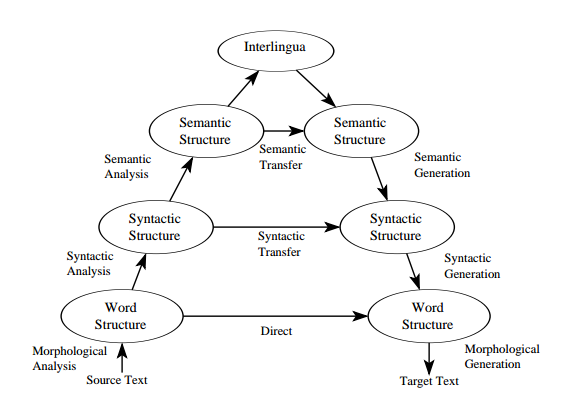
\includegraphics[scale=0.6]{Images/interlingua.png}
        \caption{Vauquois Triangle: Approaches to Machine Translation}
        \label{fig:triangle}
    \end{figure}
    
    Fig.\ref{fig:triangle}\cite{dorr} explains the approaches to MT. The higher one goes on the upward hill, the most complex is the representation. Interlingua is at the top of the figure, implies that the representation is really difficult to obtain with all the attributes in its disambiguated form. However, once the Interlingua is made, translation to target language is equally easy.
    
    So given a sentence, its interlingual representation would include the following\cite{bhattacharyya}:
    \begin{enumerate}
        \item Lexical Knowledge
        \item Structural Knowledge
        \item Discourse Knowledge
    \end{enumerate}
    
    This means its interlingual representation would include\cite{bhattacharyya}:
    \begin{enumerate}
        \item All the words in disambiguate form
        \item All words groups like multiwords
        \item All Structural ambiguities like attachment 
        \item All Discourse ambiguities like co-reference
    \end{enumerate}
    
    \subsection{Universal Networking Language (UNL): A type of Interlingua}
    UNL is an interlingua that represents information sentence by sentence. A hypergraph is made for each sentence with concepts as nodes and relations as arcs. The knowledge is primarily represented in 3-dimensions.
    \begin{enumerate}
        \item \textbf{Word Knowledge} is represented by Universal Words or UWs that are language independent. UWs are picked from lexicon during analysis phase. UWs also contains restrictions that correctly disambiguate the meaning of word. Ex: \textit{drink(icl$>$liquor)} denotes the Noun \textit{liquor}. The \textit{icl} notation indicates `inclusion' and forms an \textit{is-a} relationship.
        
        \item \textbf{Conceptual knowledge} is represented by forming a binary relation between UWs through \textit{relation labels}. There are about \num{46} relation label in UNL. A relation is typically represented as \textit{rel(UW1,UW2)}.
        
        \item Speaker's view, aspect and time are captured by attribute labels.
    \end{enumerate}
    
    \subsection{Illustration of UNL}
    \subsection{Challenges to UNL and Solution}
    Interlinguas is a universal representation of all languages as we have seen. But an important question arises. Is this knowledge repository possible? 
    \subsection{Translation Using Interlingua}
    For translation using Interlingua, only the steps of ATG process are required, since there is no transfer involved in Interlingua. First, a thorough analysis of source sentence is done to create Interlingua (A-Stage). Secondly, target sentence is generated in G-stage using syntax planning, word-ordering and functional word insertion.
    
    A sample example from \cite{bhattacharyya} is shown here to present how translation works in UNL.
    
    \begin{flushleft}
    E: On Sunday in Kolkata, Sachin donated to the cricket museum the bat with which he scored his hundredth century at Bangladesh.\\
    H: 
    \begin{hindi}
    रविवार को कोलकाता मे सचिन ने क्रि्केत सन्ग्रहलय को वह बल्ला दान कर दिया जिससे उन्होने बान्ग्लादेश मे अपना सौवा शतक लगाया| \\
    \end{hindi}
    HT: ravivaar ko kolkata mein sachin ne kriket saMgrahaalaya ko vaha ballaa daan kar diyaa jisase unhone Bangladesh mein apnaa sauwaan shatak lagaayaa thaa.
    \end{flushleft}
    
    \begin{figure}
        \centering
        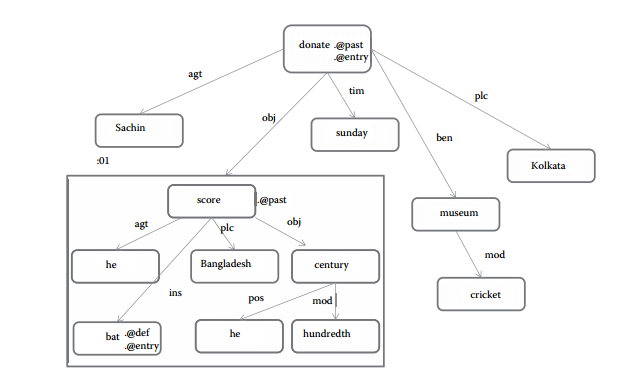
\includegraphics[scale=0.6]{Images/unl}
        \caption{UNL graph for example sentence.}
        \label{fig:unl}
    \end{figure}
    The analysis stage will:
    \begin{enumerate}
    \item Recognize named entities: Sachine(Person), Kolkata(location), Bangladesh(location)
    
    \item POS of words: On/IN Sunday/NNP in/IN Kolkata/NNP,/, Sachin/NNP donated/VBD to/TO the/DT cricket/NN museum/NN the/DT bat/NN with/IN which/WDT he/PRP scored/VBD his/PRP hundredth/JJ century/NN at/IN Bangladesh/NNP
  
    \item Get morphological information of words, i.e. \textit{donate}- main verb, past tense
    
    \item Get sense IDs of words through word sense disambiguation, i.e. \textit{donate(icl$>$give$>$do,agt$>$thing,obj$>$thing)}.
    
    \item Establish semantic relations between verb and noun, i.e. \textit{nsubj(donated-7, Sachin-6)}
    
    \item Generate attributes using grammatical properties, i.e. add .@entry and .@past attributes on donate.
    \end{enumerate}
    
    Similarly the generation stage will contain the following steps:
    \begin{enumerate}
    \item The graph corresponding to Fig.\ref{fig:unl} is parsed to record headwords, IDs, attributes and semantic relations.
    
    \item Do appropriate word mapping from lexicon. Eg: \textit{donate} $\leftrightarrow$ \textit{daan karnaa}.
    
    \item Identify case-markers for words. Eg: \textit{Kartaa Kaarak} for Sachine.
    
    \item Morphological Synthesis of words. Eg: \textit{daan karnaa} $\leftrightarrow$ \textit{daan kar diyaa}.
    
    \item Function word generation. Eg: \textit{ne} for noun Sachin, \textit{ko} for samgrahaalaya.
    \end{enumerate}
    
    \subsection{Transfer-Based MT}
    Transfer based MT is a explicit source-target pair MT, where rules are written with only source and target language in mind. It also does not insist on complete disambiguation of source sentence. 
    
    Transfer rules are typically structural transforming rules applied between a pair of languages. Transfer rules can't be generalized with any other pair of language, since they are written explicitly for each pair at a time. A transformation T can be written as\cite{bhattacharyya}:
    \begin{equation}
    T: REP_s \rightarrow REP_t
    \end{equation}
    where $REP_s$ and $REP_t$ are source and target language representation respectively. \linebreak
    Eg: E: I go to school. \\
    \quad H:
        \begin{hindi}
        मै विद्यालय जाता हूँ |\\
        \end{hindi}
       For the above example, the rules can be of the type
       \begin{equation}
    T: SVO \rightarrow SOV 
    \end{equation}
    i.e. the object and verb of the sentence should be swapped to get desired Hindi sentence output.
        
    
   	
    